\documentclass[10pt]{article}
\usepackage[polish]{babel}
\usepackage[utf8]{inputenc}
\usepackage[T1]{fontenc}
\usepackage{graphicx}
\usepackage[export]{adjustbox}
\graphicspath{ {./images/} }
\usepackage{amsmath}
\usepackage{amsfonts}
\usepackage{amssymb}
\usepackage[version=4]{mhchem}
\usepackage{stmaryrd}

\title{EGZAMIN MATURALNY Z MATEMATYKI }

\author{}
\date{}


\begin{document}
\maketitle
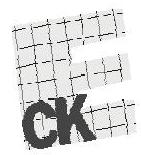
\includegraphics[max width=\textwidth, center]{2024_11_21_d9af6ed2d610d3f2d2cbg-01}\\
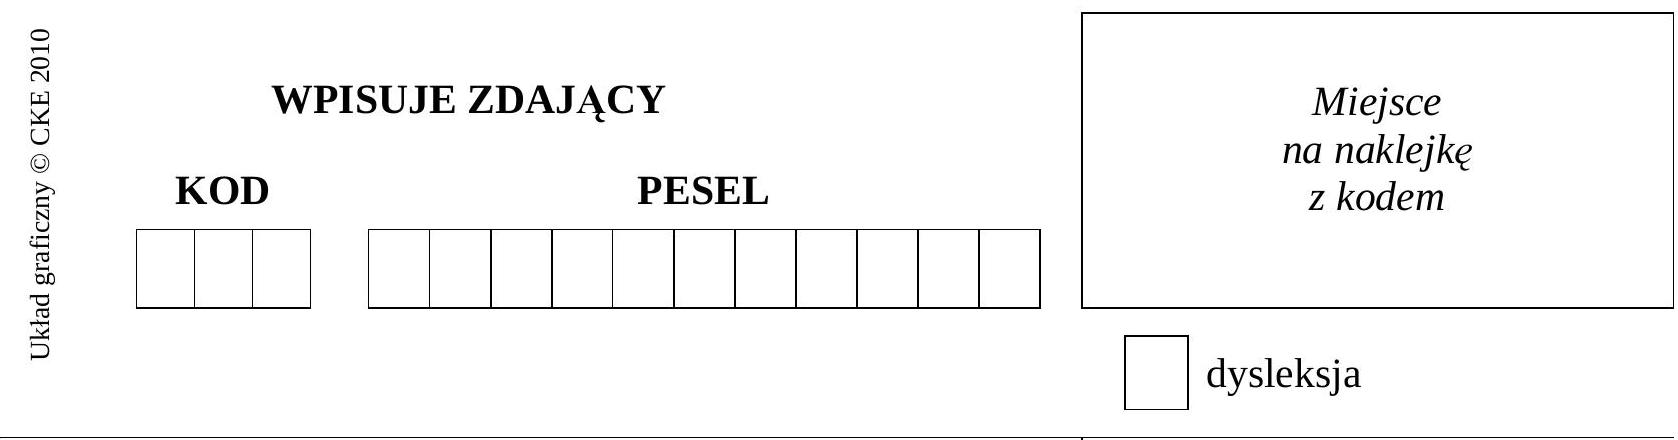
\includegraphics[max width=\textwidth, center]{2024_11_21_d9af6ed2d610d3f2d2cbg-01(1)}

CZERWIEC 2012

\section*{POZIOM ROZSZERZONY}
\begin{enumerate}
  \item Sprawdź, czy arkusz egzaminacyjny zawiera 20 stron (zadania 1-12). Ewentualny brak zgłoś
\end{enumerate}

Czas pracy: przewodniczącemu zespołu nadzorującego egzamin.\\
2. Rozwiązania zadań i odpowiedzi wpisuj w miejscu na to przeznaczonym.\\
3. Pamiętaj, że pominięcie argumentacji lub istotnych obliczeń w rozwiązaniu zadania otwartego może spowodować, że za to rozwiązanie nie będziesz mógł dostać pełnej liczby punktów.\\
4. Pisz czytelnie i używaj tylko długopisu lub pióra z czarnym tuszem lub atramentem.\\
5. Nie używaj korektora, a błędne zapisy wyraźnie przekreśl.\\
6. Pamiętaj, że zapisy w brudnopisie nie będą oceniane.\\
7. Możesz korzystać z zestawu wzorów matematycznych, cyrkla i linijki oraz kalkulatora.\\
8. Na tej stronie oraz na karcie odpowiedzi wpisz swój numer PESEL i przyklej naklejkę z kodem.\\
9. Nie wpisuj żadnych znaków w części przeznaczonej dla egzaminatora.

Liczba punktów do uzyskania: 50

MMA-R1\_1P-123

\section*{Zadanie 1. (4 pkt)}
Rozwiąż nierówność \(|x-2|+|x+1| \geq 3 x-3\).\\

\includegraphics[max width=\textwidth, center]{2024_11_21_d9af6ed2d610d3f2d2cbg-02}\\

\includegraphics[max width=\textwidth, center]{2024_11_21_d9af6ed2d610d3f2d2cbg-03}

Odpowiedź:

\section*{Zadanie 2. (4 pkt)}
Wielomian \(W(x)=x^{4}+a x^{3}+b x^{2}-24 x+9\) jest kwadratem wielomianu \(P(x)=x^{2}+c x+d\). Oblicz \(a\) oraz \(b\).\\

\includegraphics[max width=\textwidth, center]{2024_11_21_d9af6ed2d610d3f2d2cbg-04}

Odpowiedź:

\section*{Zadanie 3. (5 pkt)}
Kạt \(\alpha\) jest taki, że \(\cos \alpha+\sin \alpha=\frac{4}{3}\). Oblicz wartość wyrażenia \(|\cos \alpha-\sin \alpha|\).\\

\includegraphics[max width=\textwidth, center]{2024_11_21_d9af6ed2d610d3f2d2cbg-05}

Odpowiedź:

\section*{Zadanie 4. (5 pkt)}
Wyznacz wszystkie wartości parametru \(m\), dla których równanie \(2 x^{2}+(3-2 m) x-m+1=0\) ma dwa różne pierwiastki \(x_{1}, x_{2}\) takie, że \(\left|x_{1}-x_{2}\right|=3\).

\begin{center}
\begin{tabular}{|c|c|c|c|c|c|c|c|c|c|c|c|c|c|c|c|c|c|c|c|c|c|c|}
\hline
 &  &  &  &  &  &  &  &  &  &  &  &  &  &  &  &  &  &  &  &  &  &  \\
\hline
 &  &  &  &  &  &  &  &  &  &  &  &  &  &  &  &  &  &  &  &  &  &  \\
\hline
 &  &  &  &  &  &  &  &  &  &  &  &  &  &  &  &  &  &  &  &  &  &  \\
\hline
 &  &  &  &  &  &  &  &  &  &  &  &  &  &  &  &  &  &  &  &  &  &  \\
\hline
 &  &  &  &  &  &  &  &  &  &  &  &  &  &  &  &  &  &  &  &  &  &  \\
\hline
 &  &  &  &  &  &  &  &  &  &  &  &  &  &  &  &  &  &  &  &  &  &  \\
\hline
 &  &  &  &  &  &  &  &  &  &  &  &  &  &  &  &  &  &  &  &  &  &  \\
\hline
 &  &  &  &  &  &  &  &  &  &  &  &  &  &  &  &  &  &  &  &  &  &  \\
\hline
 &  &  &  &  &  &  &  &  &  &  &  &  &  &  &  &  &  &  &  &  &  &  \\
\hline
 &  &  &  &  &  &  &  &  &  &  &  &  &  &  &  &  &  &  &  &  &  &  \\
\hline
 &  &  &  &  &  &  &  &  &  &  &  &  &  &  &  &  &  &  &  &  &  &  \\
\hline
 &  &  &  &  &  &  &  &  &  &  &  &  &  &  &  &  &  &  &  &  &  &  \\
\hline
 &  &  &  &  &  &  &  &  &  &  &  &  &  &  &  &  &  &  &  &  &  &  \\
\hline
 &  &  &  &  &  &  &  &  &  &  &  &  &  &  &  &  &  &  &  &  &  &  \\
\hline
 &  &  &  &  &  &  &  &  &  &  &  &  &  &  &  &  &  &  &  &  &  &  \\
\hline
 &  &  &  &  &  &  &  &  &  &  &  &  &  &  &  &  &  &  &  &  &  &  \\
\hline
 &  &  &  &  &  &  &  &  &  &  &  &  &  &  &  &  &  &  &  &  &  &  \\
\hline
 &  &  &  &  &  &  &  &  &  &  &  &  &  &  &  &  &  &  &  &  &  &  \\
\hline
 &  &  &  &  &  &  &  &  &  &  &  &  &  &  &  &  &  &  &  &  &  &  \\
\hline
 &  &  &  &  &  &  &  &  &  &  &  &  &  &  &  &  &  &  &  &  &  &  \\
\hline
 &  &  &  &  &  &  &  &  &  &  &  &  &  &  &  &  &  &  &  &  &  &  \\
\hline
 &  &  &  &  &  &  &  &  &  &  &  &  &  &  &  &  &  &  &  &  &  &  \\
\hline
 &  &  &  &  &  &  &  &  &  &  &  &  &  &  &  &  &  &  &  &  &  &  \\
\hline
 &  &  &  &  &  &  &  &  &  &  &  &  &  &  &  &  &  &  &  &  &  &  \\
\hline
 &  &  &  &  &  &  &  &  &  &  &  &  &  &  &  &  &  &  &  &  &  &  \\
\hline
 &  &  &  &  &  &  &  &  &  &  &  &  &  &  &  &  &  &  &  &  &  &  \\
\hline
 &  &  &  &  &  &  &  &  &  &  &  &  &  &  &  &  &  &  &  &  &  &  \\
\hline
 &  &  &  &  &  &  &  &  &  &  &  &  &  &  &  &  &  &  &  &  &  &  \\
\hline
 &  &  &  &  &  &  &  &  &  &  &  &  &  &  &  &  &  &  &  &  &  &  \\
\hline
 &  &  &  &  &  &  &  &  &  &  &  &  &  &  &  &  &  &  &  &  &  &  \\
\hline
 &  &  &  &  &  &  &  &  &  &  &  &  &  &  &  &  &  &  &  &  &  &  \\
\hline
 &  &  &  &  &  &  &  &  &  &  &  &  &  &  &  &  &  &  &  &  &  &  \\
\hline
 &  &  &  &  &  &  &  &  &  &  &  &  &  &  &  &  &  &  &  &  &  &  \\
\hline
 &  &  &  &  &  &  &  &  &  &  &  &  &  &  &  &  &  &  &  &  &  &  \\
\hline
 &  &  &  &  &  &  &  &  &  &  &  &  &  &  &  &  &  &  &  &  &  &  \\
\hline
 &  &  &  &  &  &  &  &  &  &  &  &  &  &  &  &  &  &  &  &  &  &  \\
\hline
 &  &  &  &  &  &  &  &  &  &  &  &  &  &  &  &  &  &  &  &  &  &  \\
\hline
 &  &  &  &  &  &  &  &  &  &  &  &  &  &  &  &  &  &  &  &  &  &  \\
\hline
 &  &  &  &  &  &  &  &  &  &  &  &  &  &  &  &  &  &  &  &  &  &  \\
\hline
 &  &  &  &  &  &  &  &  &  &  &  &  &  &  &  &  &  &  &  &  &  &  \\
\hline
 &  &  &  &  &  &  &  &  &  &  &  &  &  &  &  &  &  &  &  &  &  &  \\
\hline
 &  &  &  &  &  &  &  &  &  &  &  &  &  &  &  &  &  &  &  &  &  &  \\
\hline
 &  &  &  &  &  &  &  &  &  &  &  &  &  &  &  &  &  &  &  &  &  &  \\
\hline
 &  &  &  &  &  &  &  &  &  &  &  &  &  &  &  &  &  &  &  &  &  &  \\
\hline
\end{tabular}
\end{center}

\begin{center}

\includegraphics[max width=\textwidth]{2024_11_21_d9af6ed2d610d3f2d2cbg-07}
\end{center}

Odpowiedź:

\section*{Zadanie 5. (5 pkt)}
W ciagu arytmetycznym \(\left(a_{n}\right)\), dla \(n \geq 1\), dane są \(a_{1}=-2\) oraz różnica \(r=3\). Oblicz największe \(n\) takie, że \(a_{1}+a_{2}+\ldots+a_{n}<2012\).\\

\includegraphics[max width=\textwidth, center]{2024_11_21_d9af6ed2d610d3f2d2cbg-08}

Odpowiedź:

\section*{Zadanie 6. (3 pkt)}
Udowodnij, że dla dowolnych liczb dodatnich \(a, b, c\) i \(d\) prawdziwa jest nierówność \(a c+b d \leq \sqrt{a^{2}+b^{2}} \cdot \sqrt{c^{2}+d^{2}}\).\\

\includegraphics[max width=\textwidth, center]{2024_11_21_d9af6ed2d610d3f2d2cbg-09}

\section*{Zadanie 7. (4 pkt)}
Okrąg jest styczny do osi układu wspórzzędnych w punktach \(A=(0,2)\) i \(B=(2,0)\) oraz jest styczny do prostej \(l\) w punkcie \(C=(1, a)\), gdzie \(a>1\). Wyznacz równanie prostej \(l\).\\

\includegraphics[max width=\textwidth, center]{2024_11_21_d9af6ed2d610d3f2d2cbg-10}\\

\includegraphics[max width=\textwidth, center]{2024_11_21_d9af6ed2d610d3f2d2cbg-11}

Odpowiedź:

\section*{Zadanie 8. (5 pkt)}
W czworokącie \(A B C D\) dane są długości boków: \(|A B|=24,|C D|=15,|A D|=7\). Ponadto kąty \(D A B\) oraz \(B C D\) są proste. Oblicz pole tego czworokąta oraz długości jego przekątnych.\\

\includegraphics[max width=\textwidth, center]{2024_11_21_d9af6ed2d610d3f2d2cbg-12}\\

\includegraphics[max width=\textwidth, center]{2024_11_21_d9af6ed2d610d3f2d2cbg-13}

Odpowiedź:

\section*{Zadanie 9. (3 pkt)}
Oblicz, ile jest liczb naturalnych trzycyfrowych podzielnych przez 6 lub podzielnych przez 15.\\

\includegraphics[max width=\textwidth, center]{2024_11_21_d9af6ed2d610d3f2d2cbg-14}

Odpowiedź:

\section*{Zadanie 10. (4 pkt)}
Na płaszczyźnie dane są punkty \(A=(3,-2)\) i \(B=(11,4)\). Na prostej o równaniu \(y=8 x+10\) znajdź punkt \(P\), dla którego suma \(|A P|^{2}+|B P|^{2}\) jest najmniejsza.\\

\includegraphics[max width=\textwidth, center]{2024_11_21_d9af6ed2d610d3f2d2cbg-15}

Odpowiedź:

\section*{Zadanie 11. (5 pkt)}
Podstawą ostrosłupa \(A B C S\) jest trójkąt równoramienny \(A B C\), w którym \(|A B|=30\), \(|B C|=|A C|=39\) i spodek wysokości ostrosłupa należy do jego podstawy. Każda wysokość ściany bocznej poprowadzona z wierzchołka \(S\) ma długość 26. Oblicz objętość tego ostrosłupa.\\

\includegraphics[max width=\textwidth, center]{2024_11_21_d9af6ed2d610d3f2d2cbg-16}\\

\includegraphics[max width=\textwidth, center]{2024_11_21_d9af6ed2d610d3f2d2cbg-17}

Odpowiedź:

\section*{Zadanie 12. (3 pkt)}
Zdarzenia losowe \(A\), \(B\) są zawarte w \(\Omega\) oraz \(P\left(A \cap B^{\prime}\right)=0,1\) i \(P\left(A^{\prime} \cap B\right)=0\), 2. Wykaż, że \(P(A \cap B) \leq 0,7\) ( \(A^{\prime}\) oznacza zdarzenie przeciwne do zdarzenia \(A, B^{\prime}\) oznacza zdarzenie przeciwne do zdarzenia \(B\) ).\\

\includegraphics[max width=\textwidth, center]{2024_11_21_d9af6ed2d610d3f2d2cbg-18}\\

\includegraphics[max width=\textwidth, center]{2024_11_21_d9af6ed2d610d3f2d2cbg-19}

Odpowiedź:

\section*{BRUDNOPIS}

\end{document}